\documentclass[a4paper]{article}
\author{K.A. Blondino}
\title{Magnetic Configuration of TJ-II}

\usepackage{fullpage, amsmath, graphicx, indentfirst}
\usepackage{natbib, url}
%\usepackage{lipsum}
\usepackage{float}

\linespread{1.05}


% MY NOTES IN COLOR
\usepackage{xcolor}
\newcommand\mynotes[1]{\textcolor{red}{#1}}
%\renewcommand\mynotes[1]{}

\begin{document}
\maketitle

\mynotes{What about the order of the sections? Hardware could be first or second, instead.}

\section*{Introduction}
Any fusion device that uses toroidal magnetic confinement must introduce rotational transform (poloidal twist) to mitigate particle drifts.
One approach is to create a poloidal magnetic field by having current run toroidally in the plasma, which is defined as a tokamak.
Another is the intentional wobble of the field lines in resonance with non-circular deformations of the magnetic surfaces.
A third approach, which is used by TJ-II, is a torsion of the magnetic axis, denoted as a heliac \cite{boozer_what_1998}.
The variety of stellarator concepts differ by the magnetic parameters chosen, in addition to rotational transform, such as magnetic shear, aspect ratio, symmetry of the field strength, and others \cite{iaea_fusion_2012}.
The construction and design of TJ-II is in a manner that allows for the investigation of transport and confinement of a wide range of different magnetic configurations due to its magnetic flexibility.

%---------------------------------------

\section*{Heliac Design}
There are two possible coil configurations to create a heliac.
One approach is to have the toroidal current in a tokamak produced instead by a coil, with a large enough current to produce a $q = 1$ surface.
Then, a helical coil should be wound around the outside of the torus along a path that is parallel to a field where the $q = 1$ surface would be.
The $q = 1$ surface is then split by the $m = 1$ island, in which field lines on the interior of the island form toroidal surfaces with no current.
This is the method used for TJ-II.
The second approach involves excluding a helical coil, and instead displaces the toroidal field coils helically\cite{boozer_what_1998}.
These methods cause the magnetic axis to be helical, as can be seen by the central displacement between each image in Fig. \ref{fig:cross-sections}.

\begin{figure}
%\hrule
%\vrule
\centering
\begin{minipage}{0.49\linewidth}
	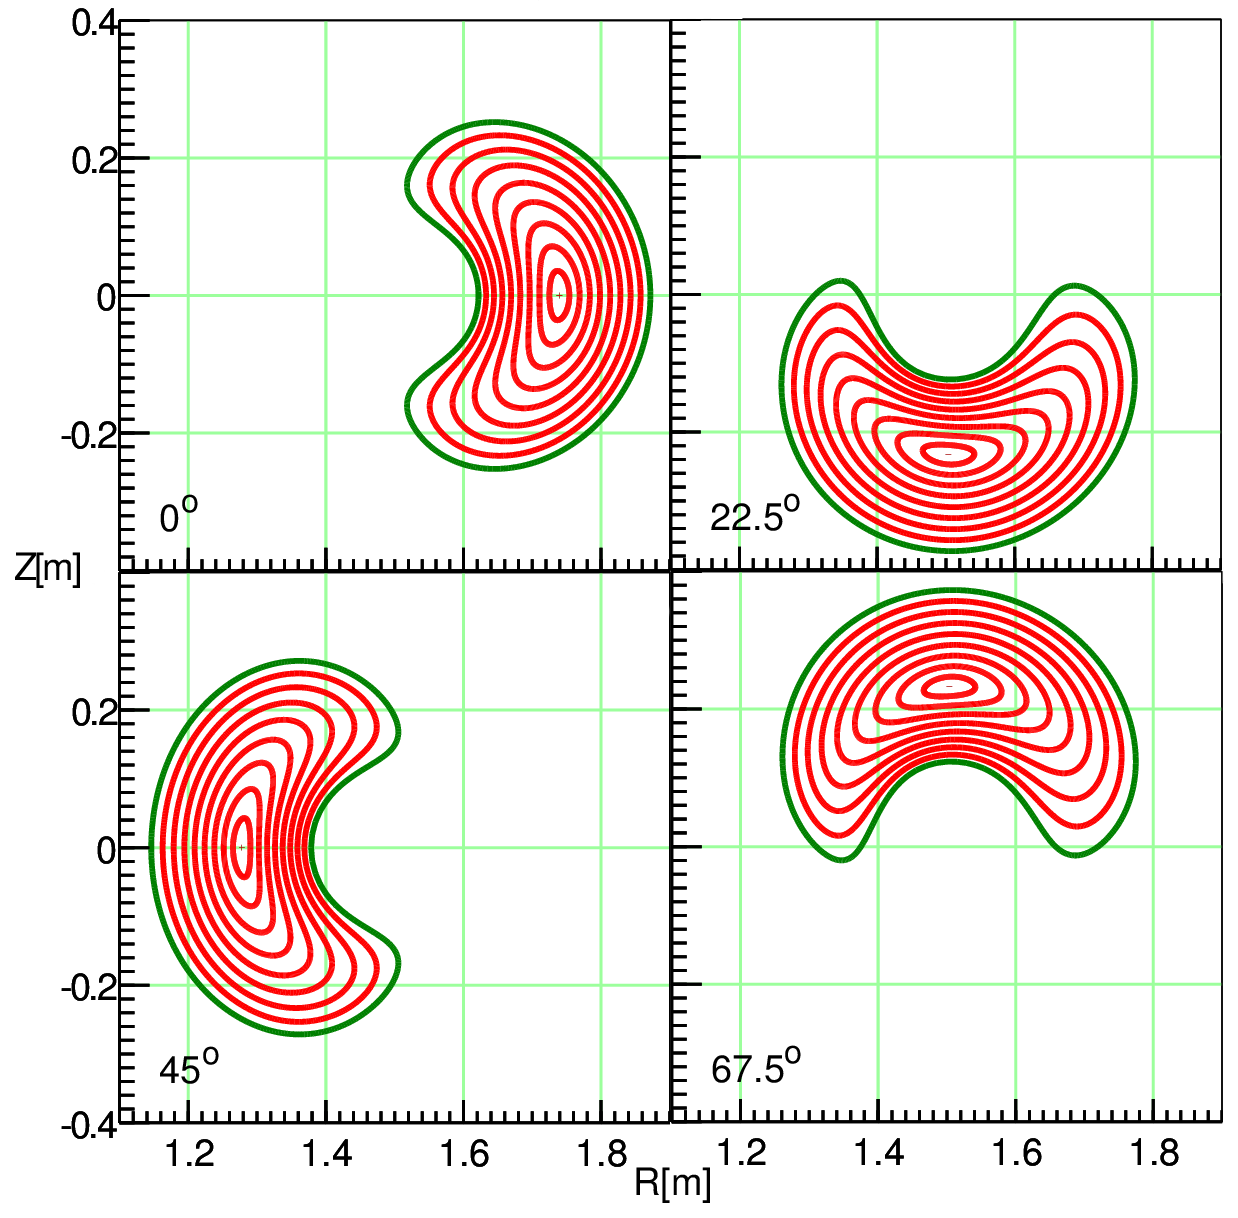
\includegraphics[width=\linewidth]{../Graphics/flux_surfaces.png}
	\caption{Flux surfaces at different toroidal angles within one toroidal period, courtesy of VMEC.}
	\label{fig:cross-sections}
\end{minipage}
\hfill\vrule\hfill
\begin{minipage}{0.48\textwidth}
	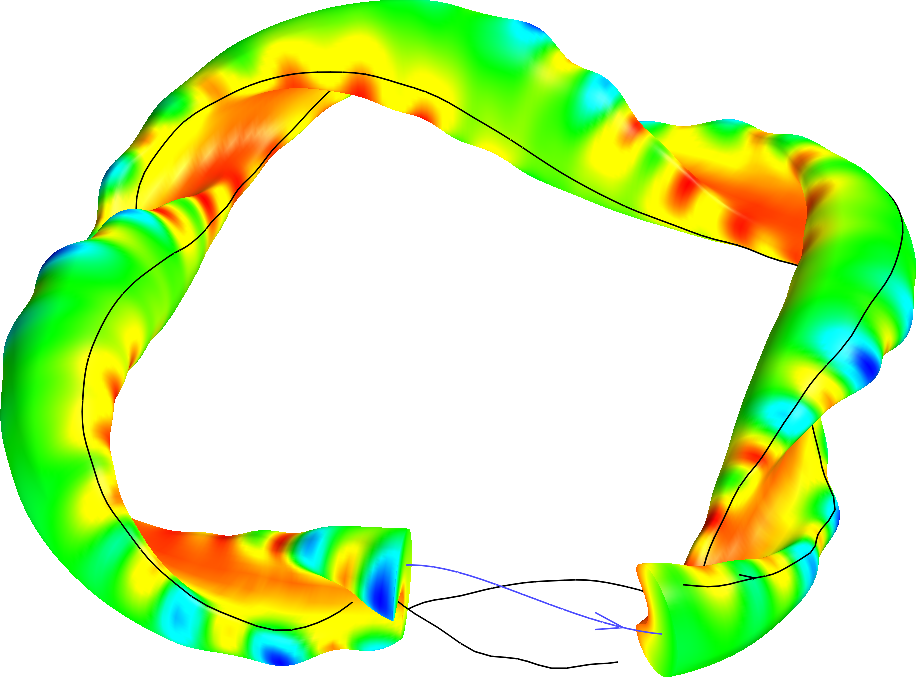
\includegraphics[width=\linewidth]{../Graphics/magnetic_field_2.png}
	\caption{Outermost magnetic surface showing higher field strengths in red and lower in blue, courtesy of VMEC. Magnetic ripple is very apparent.}
	\label{fig:magnetic_surface}
\end{minipage}
%\vrule
%\hrule
\end{figure}

For stellarators, it is impossible to reduce the solution space of the MHD equilibrium from three to two dimensions, as all stellarators are non-axissymetric.
However, various designs do allow for quasisymmetry, in which the \emph{magnitude} of the magnetic field can depend on only one angular coordinate:
\begin{equation}
	B \,=\, B(\psi,\,\theta - N_p\phi) \,=\, B(\psi,\,\Theta)
\end{equation}

If $N_p$, an integer, is zero, it is said that the device is quasi-axissymetric; otherwise, it has quasihelical symmetry.
The direction of the magnetic field, however, still depends on at least three spatial coordinates.
Quasisymmetry has the benefit of causing neoclassical transport to be similar to that of a tokamak, reduced as compared to stellarators lacking quasisymmetry \cite{boozer_what_1998}.
It is integral to note that TJ-II, as all heliac-designed stellarators, is not quasisymmetric.

\mynotes{Perhaps explain more of quasisymmetry and move the next small paragraph to flexibility section.}

However, TJ-II has very low magnetic shear \cite{milligen_mhd_2012}.
This means that the rotational tranform profile $\iota(\psi)$ is purposely kept nearly flat in order to avoid large magnetic islands.
Devices with low shear generally have magnetic wells, which is an additional stabilizing mechanism \cite{aguilera_magnetic_2015}.

%---------------------------------------

\section*{Fourier Representation and Flexibility}
Any toroidal magnetic configuration can be described by the Fourier components of the field in Boozer coordinates, shown in the following equation:
\begin{equation*}
	B \,=\, B_0 \sum_{m,n} a_{m,n}\left(\psi\right) \cos\left(m\theta - n\phi\right),
\end{equation*}
where $\theta$ and $\phi$ are the poloidal and toroidal angles, $m$ and $n$ are integers, and $a_{m,n}$ are the coefficients.

In the TJ-II design, it was found that four of these coefficients are dominant harmonics.
These are the toroidicity $a_{0,-1}$, the helicity $a_{4,1}$, the magnetic ripple $a_{32,0}$, and the corner ripple $a_{4,0}$.
Figure~\ref{fig:topology} \mynotes{(HELP!)} shows the topology of the magnetic field with three of the four dominant harmonics, allowing for the visualization of each harmonic. The field is broken down as the following equation \cite{solano_study_1988}:
\begin{equation}
	B \,=\,B_0\left[1 + a_{0,-1}\cos\theta + a_{4,1}\cos\left(4\theta - \phi\right) + a_{4,0}\cos\left(4\phi\right)\right].
\end{equation}

The helicity term causes the field to approach the direction of the helical coils; the corner ripple term produces a minimum at $\theta = 0^{\circ}, \phi = 0^{\circ}$.
The inclusion of the magnetic ripple harmonic produces large wiggles in the topology \cite{solano_study_1988}.

One method in adjusting the magnetic configuration is by modulating the current in the toroidal field (TF) coils.
For example, giving a spatially sinusoidally-changing current as follows,
\begin{equation}
	I(\phi) \,=\, I_0 \left[1 + c_P\cos(4 \phi)\right],
\end{equation}
one changes the magnitude of the corner ripple, depending on the amplitude $c_P$.
In addition, the rotational transform $\iota$ can also be modified by adjusting the current in all the coils \cite{solano_study_1988}.

\begin{figure}
\centering
	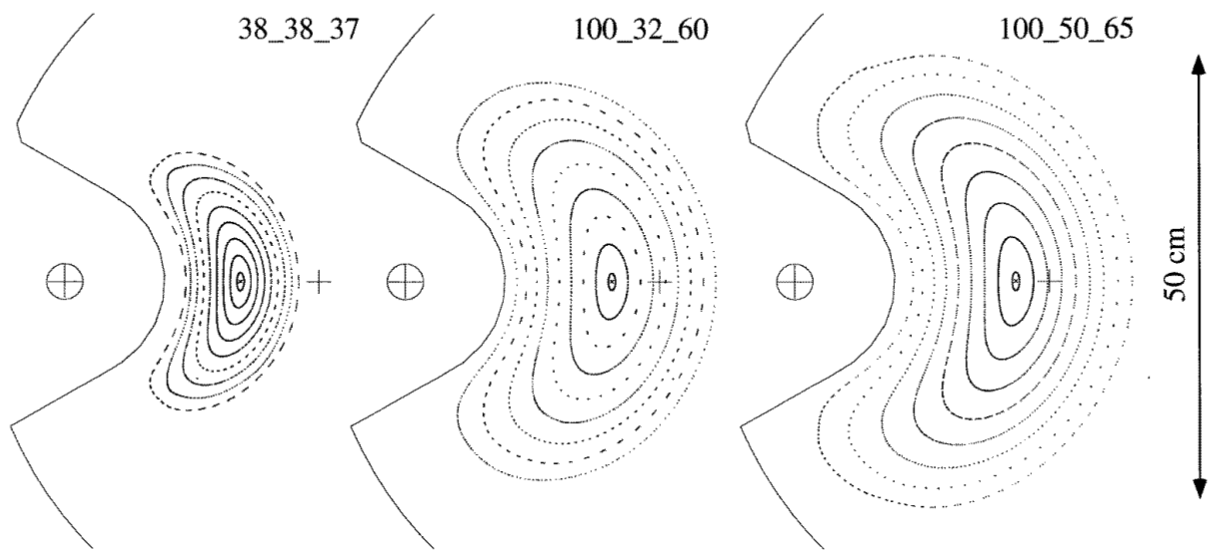
\includegraphics[width=\linewidth]{../Graphics/3_configs.png}
	\caption{Vacuum flux surfaces at the toroidal angle $\phi = 0$ for three configurations. A variety of physical quantities can be varied, such as plasma volume and rotational transform \cite{alejaldre_first_1999}.}
	\label{fig:3_configs}
\end{figure}

%---------------------------------------

\section*{Hardware}
The basic dimensions of the machine includes a major radius of 1.5 m and an averaged minor radius of 0.2 m. The magnetic system of TJ-II consists of 44 individual coils in total, shown in Fig.~\ref{fig:coils}.
The main helical field is produced by the circular coil (CC), the helical coil (HX), and the 32 toroidal field coils (shown in red, yellow, and blue, respectively) \cite{tj-ii_nodate}.

Because the helical coil spirals around the outer stainless-steel casing of the circular coil, special care was needed for installation.
In addition, the helical coil is composed of two subcoils with 12 windings, with individually supplied currents, allowing for shear variation.
The circular and helical coils have a maximum current of 280 kA and 260 kA, respectively.
Together, they give a maximum current density of 120 MA/m$^2$.
The 32 TF coils have a maximum field strength of 1 T.
To mitigate magnetic ripple, the TF coils' currents are modulated.
Assembly required the coils, as well as their support structures, to be built in halves \cite{ascasibar_overview_2001}.

TJ-II is considered a ``flexible'' heliac because the magnetic configuration can be changed by adjusting the currents in the toroidal and central coils \cite{solano_study_1988}.
In addition, each system is mechanically de-coupled, each having its own support structure \cite{ascasibar_overview_2001}.
This allows for study in the effects of different configurations.
Specifically, in addition to the plasma volume and radius, the rotational transform can be varied.
As it is a heliac, the overall shape of the cross-section does not change; the ``bean''-shaped cross-section is shown in Fig.~\ref{fig:cross-sections}.

\begin{figure}[tb]
%\hrule
%\vrule
\centering
\begin{minipage}{0.5\linewidth}
	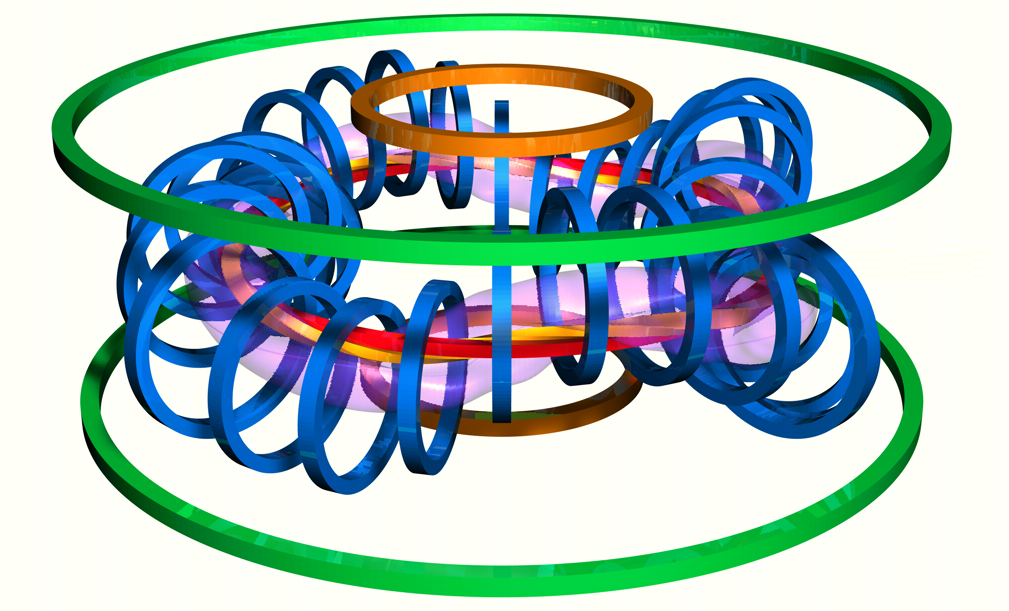
\includegraphics[width=\linewidth]{../Graphics/TJ-II_Coils.png}
	\caption{Color-labeled coils of TJ-II that recreate the magnetic surface. Red: circular, yellow: helical, blue: toroidal, green: vertical, brown: radial \cite{tj-ii_nodate}.}
	\label{fig:coils}
\end{minipage}
\hfill\vrule\hfill
\begin{minipage}{0.46\linewidth}
	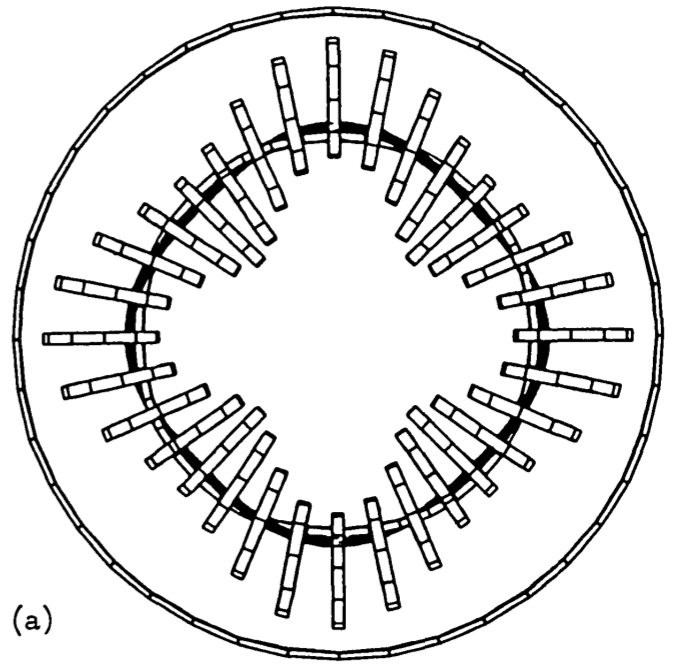
\includegraphics[width=\linewidth]{../Graphics/TJ-II_overhead.png}
	\caption{Overhead view of TJ-II, showing the circular, helical, and vertical coils and all 32 toroidal field coils \cite{solano_study_1988}.}
	\label{fig:coils}
\end{minipage}
%\vrule
%\hrule
\end{figure}

%---------------------------------------

\section*{Conclusion}
TJ-II's magnetic configuration is that of a low-magnetic shear heliac with magnetic wells.
It was chosen to use a circular and helical coil to generate the torsion of the magnetic axis, in conjunction with 32 toroidal field coils.
Additionally, these coils, along with shaping coils, allow for great flexibility in the exact specifications of the configuration.
This allows for a wide variety of investigation in confinement and transport in heliac design.
The device lacks any kind of quasisymmetry. Nevertheless, analysis of its magnetic topology has been done by representing the field as a Fourier series. \mynotes{This needs SERIOUS improvements.}

%---------------------------------------

% References
%\newpage
\bibliographystyle{plain}
%\nocite{*}
\bibliography{../References/References}
\end{document}
